
\section{Calculating Reputation: Miners and Merkle Proofs}\label{sec:reputationmining}
The reputation system is a core component of any decentralised colony. By carefully balancing the rewards and penalties we aim to keep every users' incentives aligned with the colony and the colony network. Since reputation can only be \emph{earned} and not transferred between accounts, the system fosters a more meritocratic form of decision making than pure token-weighted voting can hope to achieve. The continuous decay of reputation ensures that the influence conveyed by reputation is recently earned and up-to-date. As such, it prevents a reputation aristocracy and allows for a fluid passing of control from one set of contributors to another over time.


Due to the combined complexity of reputation scores across multiple colonies, domains, and skills, reputation scores cannot be stored or calculated on-chain. Instead, the calculations will all take place off-chain, the results of which will be reported to the blockchain by participating CLNY holders --- in a process resembling a proof-of-stake blockchain consensus protocol. We call this procedure \textbf{`Reputation Mining'}.

The reputation calculation whose result the miners are submitting is determined by the activities that have taken place in the colonies and can be fully deterministically derived from the ethereum blockchain. Game-theoretically the system is protected similarly to the off-chain calculations of TrueBit (\cite{TruebitWhitepaper}) in that, \emph{while the calculation cannot be done on-chain and a correct submission can never be proved true, an incorrect calculation can always be proved to be wrong}.


\subsection{Merkle Trees and Proofs}\label{sec:Merkle-summary}
This subsection contains only a summary of Merkle trees (\cite{MerkleTrees}, \cite{MerkleInEthereum}) and Merkle proofs in order to establish some terminology, and can be skipped if already familiar with them.

Consider the tree shown in Figure \ref{fig:Merkleexample}. The data leaves of the tree (1, 2, 3 and 4) are each hashed individually to give A, B, C and D. These are then repeatedly hashed pairwise until only a single hash remains, indicated by G in Figure \ref{fig:Merkleexample}. In the event of a starting or an intermediate array being an odd number (which will always happen for a starting array that is not a power of two), the hash contained in the last element is hashed with itself.

The resulting structure is known as a Merkle tree. In order to prove that the element \ascode{1} is in the tree with root \ascode{G}, one submits a Merkle proof containing the information \ascode{1, [B,F], [l,l]}. The first argument is the element whose existence is to be proved. The second argument is the list of hashes that the hash of the first element should be hashed with in succession. The last argument is an array of \ascode{l}'s and \ascode{r}'s that indicates whether the hash calculated so far should be hashed on the left or the right of next element in question. So to show that \ascode{3} was in the tree with root \ascode{G}, the proof would be of the form \ascode{3, [D,E], [l,r]}.
\begin{figure}
\centering
 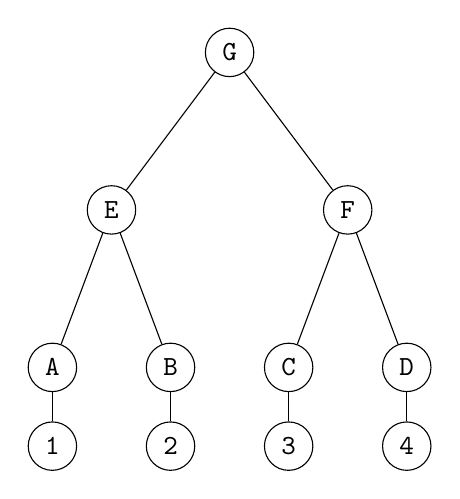
\begin{tikzpicture}
  \node[shape=circle, draw] at (0,-4) (a) {\texttt{A}};
  \node[shape=circle, draw] at (0,-5) (1) {\texttt{1}}
   edge[-] (a);
  \node[shape=circle, draw] at (1.5,-4) (b) {\texttt{B}};
  \node[shape=circle, draw] at (1.5,-5) (2) {\texttt{2}}
   edge[-] (b);

  \node[shape=circle, draw] at (3,-4) (c) {\texttt{C}};
  \node[shape=circle, draw] at (3,-5) (3) {\texttt{3}}
   edge[-] (c);
  \node[shape=circle, draw] at (4.5,-4) (d) {\texttt{D}};
  \node[shape=circle, draw] at (4.5,-5) (4) {\texttt{4}}
   edge[-] (d);
  %
  \node[shape=circle, draw] at (0.75,-2) (e) {\texttt{E}}
   edge[-] (a)
   edge[-] (b);
  \node[shape=circle, draw] at (3.75,-2) (f) {\texttt{F}}
   edge[-] (c)
   edge[-] (d);
  %
  \node[shape=circle, draw] at (2.25,0) (g) {\texttt{G}}
   edge[-] (e)
   edge[-] (f);
 \end{tikzpicture}
 \caption{A simple Merkle tree. Elements A, B, C and D correspond to the hashes of 1, 2, 3 and 4. E is the hash of A concatenated with B.}
 \label{fig:Merkleexample}
\end{figure}

Note also that the array of \ascode{l}'s and \ascode{r}'s nothing more than a binary representation of the leaf node's index in the tree. When expressed in this way, we refer to the index as the `path' in the Merkle proof. We refer to the objects that get hashed along the way (i.e. \ascode{D} and \ascode{E}) as the `siblings'.


\subsection{The Reputation Tree and the ReputationRootHash}\label{sec:reptree}
The data leaves in the reputation tree are the reputations all users have in all skills, as well as the colony-wide totals. Such a leaf consists of the following data:
\[
R =
\begin{cases}
 \ascode{rep\_id} & \textnormal{the id of a skill or domain identifying the type of reputation},\\
 \ascode{colony\_id} & \textnormal{the colony the reputation is held in},\\
 \ascode{user} & \textnormal{the address holding the skill},\\
 \ascode{amount} & \textnormal{the numerical value of the reputation}.
\end{cases}
\]

All individual reputations are assembled into the \textbf{``Reputation Tree''} which is a Merkle tree of all individual reputations in a colony, as well as the total reputation of each type held by the users in each colony. The leaves that represent these colony-wide totals are indicated by setting \ascode{user} to zero. These leaves are then put into a Merkle tree in the usual way (described in Section \ref{sec:Merkle-summary}).\footnote{The ordering of the data leaves is only determined by when these reputations were first earned.} We term the root hash of the resulting tree the \ascode{ReputationRootHash}, $\mathcal{RH}$.
\begin{figure}
\centering
\begin{tikzpicture}
 \node at (0,-5) (r0) {$R_0$};
 \node at (1.5,-5) (r1) {$R_1$};
 \node at (3,-5) (r2) {$R_2$};
 \node at (4.5,-5) (r3) {$R_3$};
 \node at (6,-5) (rdots) {$\cdots$};
 \node at (8,-5) (rn) {$R_N$};
 %
 \node at (0,-4) (r0hash) {$\mathcal{H}(R_0)$}
  edge[-] (r0);
 \node at (1.5,-4) (r1hash) {$\mathcal{H}(R_1)$}
  edge[-] (r1);
 \node at (3,-4) (r2hash) {$\mathcal{H}(R_2)$}
  edge[-] (r2);
 \node at (4.5,-4) (r3hash) {$\mathcal{H}(R_3)$}
  edge[-] (r3);
 \node at (8,-4) (rnhash) {$\mathcal{H}(R_N)$}
  edge[-] (rn);
 %
 \node at (0.75,-2.5) (r01) {$\mathcal{H}_{0,1}$}
  edge[-] (r0hash)
  edge[-] (r1hash);
 \node at (3.75,-2.5) (r23) {$\mathcal{H}_{2,3}$}
  edge[-] (r2hash)
  edge[-] (r3hash);
 \node at (7,-2.5) (rnn) {$\mathcal{H}_{N-1,N}$}
  edge[-] (rnhash)
  edge[dashed] (6.5,-4);
 %
 \node at (2.25,-1) (r14) {$\mathcal{H}_{0,3}$}
  edge[-] (r01)
  edge[-] (r23);
 %
 \node[draw, fill=gray!5] at (4,0) (root) {\texttt{ReputationRootHash}  ($\mathcal{RH}$)};
 \node[below = 1mm of root] (dummy) {\phantom{a}}
  (dummy.north west) edge[dashed] (r14)
  (dummy.north east) edge[dashed] (rnn);
 %
 %
\end{tikzpicture}
\caption{The Merkle tree of users' reputations with \ascode{ReputationRootHash} as the root. We use $\mathcal{H}$ to indicate the \ascode{keccak256} hash function. Above the second row, each element is the hash of the concatenation of its two children.}
\end{figure}


The \ascode{ReputationRootHash} is the only data we record on the blockchain associated with users' reputations. It summarises the state of the whole reputation system and whenever a user wishes to make use of their reputation, they can submit a Merkle proof from the reputation $\mathcal{R}_i$ they wish to make use of and ending at $\mathcal{RH}$.

\subsection{Calculating the new root hash}
To calculate the new root hash, the miners begin with the last reputation state, and decay all reputations held by all users in all colonies, in the order of the leaves in the tree. They then take the set of reputation gains or losses that were not in the last state submitted, and are to be included in the next state. They apply the reputation updates to each user in each colony, updating or adding leaves as necessary, to end up with a new list of reputations for all users and colonies. These new reputations are then hashed and assembled into a new Merkle tree yielding an updated \ascode{ReputationRootHash}.

While the calculation is too large to be done on-chain due to technical and economic limitations (i.e. the block gas limit and the cost of gas, respectively), this calculation can easily be performed by a typical user's computer.

\subsection{Submission of a new root hash}
%
\subsubsection*{What is submitted?}
The final \ascode{ReputationRootHash} is submitted to the contract by the miner along with the number of leaves in the tree. Further, the miner also submits the IPFS or Swarm hash of a document containing the entire state tree, though this is only for convenience; any user can construct this locally based on the blockchain history.
%
\subsubsection*{Who can submit a new root hash?}
All CLNY token holders are eligible to become miners and participate in the reputation update process, but since any user can calculate the correct root hash locally, it would be possible for \emph{any} miner to submit the hash to the contract.

It is however undesirable to have too many submissions for every update. We propose a mechanism that only allows some miners to submit results to begin with. To participate in the mining process, \rcths\ must stake some of their tokens to become `reputation miners'. A submission will only be accepted from a miner if
\begin{equation*}\label{eq:mining-difficulty}
\ascode{keccak256(address, N, hash)} < \ascode{target}.
\end{equation*}
At the beginning of the submission window, the target is set to 0 and slowly increases to $2^{256}-1$ after 150 blocks. We limit the total number of miners allowed to submit a specific hash to 12.

The variable $N$ that goes into the hash is some integer greater than 0 and less than the number of tokens the \rcth\ address has staked divided by $10^{15}$, meaning that users with a large stake have a higher chance of qualifying to submit a hash sooner than smaller stake holders. The factor of $10^{15}$ is introduced to ensure that all hashes a user is eligible to submit can be calculated in a few seconds by the client. It also effectively creates a minimum number of tokens that must be staked to submit a hash. This puts a tangible cost on any attacks revolving around spamming known false submissions (see Section \ref{sec:mining-possible-attacks}).

Miners will also be required to have staked their tokens for a few update cycles before they are eligible to submit or support a hash.
%
\subsubsection*{Verifying a submission}
If only one state is submitted by the end of the submission period, then the new state is accepted, and proposals of the next state can begin to be made. This is expected to be the most common occurrence.

If more than one state has been submitted, then either someone has made a mistake, or there is a malicious entity trying to introduce a fraudulent reputation change. In this event, the a challenge-response protocol can establish which state is incorrect (see Section \ref{sec:challengeresponse})

\subsubsection*{Mining Rewards}

When a state is accepted, a number of (newly minted) \rcts\ are made available for the users who submitted the correct state to claim as a reward. They also receive a corresponding amount of reputation in the \rc\ (in a special mining skill, which only users in the \rc\ can earn by performing this task). This reputation update is no different from any other, aside from the limitations of who is able to earn it, and will be included in the subsequent reputation update cycle. The size of the rewards and their distribution are described in Section \ref{subsec:mining-costs-and-rewards}.

\subsection{Dealing with false submissions}\label{sec:challengeresponse}
%
\subsubsection{The Challenge-Response Protocol}

We assume that the correct hash is one of the  submitted hashes. This is a reasonable assumption, as only one out of all the miners is required to make a correct submission, and there is an incentive for them to do so (the reward defined in Section \ref{subsec:mining-costs-and-rewards}). Thus our task is not to validate the correct hash but to invalidate the false ones.

We must prove all but one submission incorrect by having each submission navigate a series of \emph{challenges}. These challenges refer to events that happened in the colony network within the last update cycle that have an effect on reputation. The \emph{responses} to the challenges are Merkle proofs that the corresponding reputation update was properly handled. Anyone is able to respond to a challenge, regardless of who submitted the original hash; this should ensure that the correct state is always defended.

We begin with the scenario where only two submissions are made, and one is correct.

First we consider the case in which the same hash has been submitted twice, but with a disagreement about the number of leaves it contained. In this situation, the users are required to submit a Merkle proof for the last leaf in their tree. We are able to tell if a submitted proof corresponds to the last leaf in the tree, as all sibling hashes must be hashed on the left. Noting the positions in the Merkle proof in which a hash is hashed with itself also allows us to tell the index of this last leaf; if it corresponds to either of the submitted states, that one is correct.

We now consider the more complicated case where two different hashes have been submitted.

\subsubsection*{1. The Justification Tree}
  \newcommand{\jrh}{\ensuremath{\mathbb{JRH}}}
The first step is for both parties to upload a justification of their submitted hash. This justification consists of a second Merkle root and two Merkle proofs.

The Merkle root in questions is the \ascode{JustificationRootHash} (\jrh); it is the root of the `Justification Tree' -- a tree where each leaf represents a complete reputation state i.e. each leaf is a \ascode{ReputationRootHash}.

The left-most leaf of the Justification Tree ($\mathcal{RH}_0$) is the final accepted reputation state from the last update. Both parties must submit a proof that their tree does indeed start at $\mathcal{RH}_0$. Note that in a Merkle proof for a left-most leaf, all siblings are hashed on the right.

The right-most leaf of the Justification Tree ($\mathcal{RH}_n$) is the \ascode{ReputationRootHash} they originally submitted. Both parties must submit a Merkle proof that their tree does indeed end with this hash. Note that in a Merkle proof for a right-most leaf, all siblings are hashes on the left; furthermore, by noting the steps at which a hash is hashed with itself, we can determine the index of the last leaf. This index is required to be $n$ --- the number of reputation updates in the log.

The intermediate leaves of the Justification Tree represent the evolution of the reputation state, with $\mathcal{RH}_i$ corresponding to the reputation state after the first $i$ reputation updates in this cycle have been applied.

 %
\begin{figure}
\centering
\begin{tikzpicture}
 \node at (0,-4) (rh0) {$\mathcal{RH}_0$};
 \node at (1.5,-4) (rh1) {$\mathcal{RH}_1$};
 \node at (3,-4) (rh2) {$\mathcal{RH}_2$};
 \node at (4.5,-4) (rh3) {$\mathcal{RH}_3$};
 \node at (6,-4) (rh4) {$\mathcal{RH}_4$};
 \node at (7,-4) (rdots) {$\cdots$};
 \node at (8,-4) (rhn1) {$\mathcal{RH}_{n-1}$};
 \node at (9.5,-4) (rhn) {$\mathcal{RH}_n$};
 %
 \node at (0.75,-2.5) (rh01) {$h_{0,1}$}
  edge[-] (rh0)
  edge[-] (rh1);
 %
 \node at (2.25,-2.5) (rh12) {$h_{1,2}$}
  edge[-] (rh1)
  edge[-] (rh2);
 %
 \node at (3.75,-2.5) (rh23) {$h_{2,3}$}
  edge[-] (rh2)
  edge[-] (rh3);
 %
 \node at (5.25,-2.5) (rh34) {$h_{3,4}$}
  edge[-] (rh3)
  edge[-] (rh4);
 %
 \node at (8.5,-2.5) (rhnn) {$h_{n-1,n}$}
  edge[-] (rhn)
  edge[-] (rhn1);
 %
 \node at (1.5,-1) (rh02) {$h_{0,2}$}
  edge[-] (rh01)
  edge[-] (rh12);
 %
 \node at (4.5,-1) (rh24) {$h_{2,4}$}
  edge[-] (rh23)
  edge[-] (rh34);
 %
 \node at (3,0) (dummy14) {$h_{0,4}$}
  edge[] (rh02)
  edge[] (rh24);
 %
 \node[draw, fill=gray!5] at (5,1) (root) {\texttt{JustificationRootHash} (\jrh)};
 \node[below = 1mm of root] (dummy) {\phantom{a}}
  (dummy.north west) edge[dashed] (dummy14)
  (dummy.north east) edge[dashed] (rhnn);
 %
 %
\end{tikzpicture}
\caption{The Justification Tree. Note that each intermediate leaf $\mathcal{RH}_i$ is hashed into the tree twice. }
\label{fig:justification-tree}
\end{figure}
An example of such a tree is shown in Figure \ref{fig:justification-tree}. Note that in the first stage of the tree, every neighbouring pair of data leaves is hashed, and so any pair has a shared Merkle proof to the root. We do this so that each element in the first row of hashes (indicated by $h_{0,1}, h_{0,2} \ldots h_{n-1,n}$ in Figure \ref{fig:justification-tree}) represents a transition between two states. It is these transitions that are the subject of the mining dispute resolution process.

Since any two differing submitted states agree on the first leaf $\mathcal{RH}_0$ (which is the \ascode{ReputationRootHash} accepted at the end of the previous iteration of the mining process), and disagree on the last leaf $\mathcal{RH}_n$ (the hash they submitted), there must be a hash ($h_{i,i+1}$) that represents the transition from $\mathcal{RH}_i$ to $\mathcal{RH}_{i+1}$) where they agree on the starting state but disagree on the result. This transition is meant to be the effect of a single reputation update (the $i^{th}$)\footnote{We start counting at zero, i.e. the transition from $\mathcal{RH}_{0}$ to $\mathcal{RH}_{1}$ is the `zeroth'.}, and this is the reputation update we will calculate on-chain to establish which submission is incorrect.\\

\noindent First, however, we must establish where the two submissions first differ.

\subsubsection*{2. Searching for the discrepancy}
The contract requires both parties to submit repeated Merkle proofs that specific reputation updates were handled correctly until the first discrepancy between the two submissions is found.

We shall call the two parties $A$ and $B$ and we shall indicate which party made a submission by a superscript of $A$ or $B$. Furthermore we introduce the simplifying notation of $\overline{h}$ to mean `sibling of $h$' in the Merkle tree. Recall that if $h$ does not have an immediate sibling, $\overline{h}$ is taken to be equal to $h$ as per our rule of hashing these elements with themselves.

Along with their justification root hashes $\jrh^A$ and $\jrh^B$ both parties have already submitted proofs for the left-most leaf. These proofs have the simplified\footnote{Since we know that the proofs concern the first and last leaf of the tree, no array of left-right information is needed.} form:
\[
 \overline{\mathcal{RH}_0}^A, \overline{h_{0,1}}^A, \overline{h_{0,2}}^A, \ldots \overline{h_{0,2^k}}^A \qquad \textnormal{ terminating at } \jrh^A
\]
and
\[
 \overline{\mathcal{RH}_0}^B, \overline{h_{0,1}}^B, \overline{h_{0,2}}^B, \ldots \overline{h_{0,2^k}}^B \qquad \textnormal{ terminating at } \jrh^B
\]
where $k$ is the largest integer such that $2^k$ is smaller than $n$.

When the first miner (say $A$) submits their proof the contract saves the values of $h_{0,2^k}^A$ and $\overline{h_{0,2^k}}^A$. When the second miner submits their proof the contract compares $h_{0,2^k}^A$ to $h_{0,2^k}^B$. If they are not equal, the contract saves both of these values (and forgets $\overline{h_{0,2^k}}^A$). If they are equal, the contract retains the values of $\overline{h_{0,2^k}}^A$ and $\overline{h_{0,2^k}}^B$ (forgetting $h_{0,2^k}^A$).

The rationale behind this behaviour is the following: If $h_{0,2^k}^A = h_{0,2^k}^B$ then the two justification trees are equal between $\mathcal{RH}_0$ and $\mathcal{RH}_{2^{k-1}}$ and the first discrepancy must lie in the right-hand subtree whose root is $\overline{h_{0,2^k}}^A$ for miner $A$ and $\overline{h_{0,2^k}}^B$ for miner $B$. If on the other hand $h_{0,2^k}^A \neq h_{0,2^k}^B$, then the first discrepancy must lie in the left-hand subtrees given by $h_{0,2^k}^A$ and $h_{0,2^k}^B$. The situation is summarised by
\begin{eqnarray*}
 h_{0,2^k}^A \neq h_{0,2^k}^B & \Longrightarrow & \textnormal{First discrepancy occurs at some } \mathcal{RH}_i \textnormal{ with } 0 \leqslant i < 2^k\\
 h_{0,2^k}^A = h_{0,2^k}^B & \Longrightarrow & \textnormal{First discrepancy occurs at some } \mathcal{RH}_i \textnormal{ with } 2^k \leqslant i < n
\end{eqnarray*}

The contract begins its search by %pseudorandomly%\footnote{This pseudorandomness is to help mitigate an attack described in Section \ref{sec:mining-possible-attacks}.}
%picking an index $j$ from within the range the first discrepancy in known to lie in. It then
%
picking an index $j$ from within the range the first discrepancy in known to lie in (say always the smallest), and requiring both parties to provide a Merkle proof showing how the $j^{th}$ reputation update from all updates to be applied this cycle (Section \ref{subsec:reputation-update-log}) was included in their justification tree. The required target of this proof is no longer the $\jrh$ itself, but rather the retained value for $h_{0,2^k}$ or $\overline{h_{0,2^k}}$. Specifically this proof consists of

\begin{itemize}
 \item[(i)] The root hash before the update was applied ($\mathcal{RH}_{j}$).
 \item[(ii)] The root hash after the update was applied ($\mathcal{RH}_{j+1}$).
 \item[(iii)] A Merkle proof showing the inclusion of $h_{j,j+1}$ in the relevant justification sub-tree.
\end{itemize}

The same process as before of comparing hashes and retaining the roots of either the left-side subtree or the right-side subtree is repeated. With each iteration, the range of possible values for the index of the first discrepancy is reduced by (on average) a factor of two and the length of the required Merkle proofs is reduced by one.

% and requires both parties to provide:
% \begin{itemize}
%  \item[(i)] The root hash before the update was applied ($\mathcal{RH}_{i-1}$).
%  \item[(ii)] The root hash after the update was applied ($\mathcal{RH}_i$).
%  \item[(iii)] A Merkle proof showing that the pair ($\mathcal{RH}_{i-1}, \mathcal{RH}_i$) is correctly included in the justification tree.
% \end{itemize}
%
% When either party submits, first their Merkle proof is checked. It must use the correct sequence of \ascode{l} and \ascode{r} during the hashing process, which is defined by the $i$ that has been selected. If the Merkle proof is correct, then if this is the first party to submit, their $\mathcal{RH}^A_{i-1}$ and $\mathcal{RH}^A_{i}$ are stored. We label these with a superscript `A' to denote they have come from the first party to submit.
%
% When the second party submits and their Merkle proof is found valid, then the contract compares the submitted $\mathcal{RH}^B_{i-1}$ and $\mathcal{RH}^B_{i}$ to $\mathcal{RH}^A_{i-1}$ and $\mathcal{RH}^A_{i}$ stored from the first party's submission.
%
% If the pairs of submitted root hashes are identical, the (first) discrepancy between the two calculations occurs must occur later in the tree. The lower bound for the search for the first discrepancy can be set to $i+1$. If the submitted root root hashes are such that $\mathcal{RH}^A_{i-1}\neq\mathcal{RH}^B_{i-1}$ and $\mathcal{RH}^A_{i}\neq\mathcal{RH}^B_{i}$, then the first discrepancy must occur later in the tree. The upper bound for the search can be set to $i-2$.
%
% This process repeats, pseudorandomly selecting a new $i$ within the still-valid bounds of the search for the new challenge. Each newly submitted proof further reduces the size of the search space by a factor of two on average.\footnote{By examining precisely at which sibling the first discrepancy occurs, some stages of the binary search could be skipped. However, in order to accomplish this all the siblings of the proof that first completed the challenge would need to be stored on the blockchain, so it is more gas efficient to do the na\"{i}ve binary search for all but the very smallest of trees.}

There are two ways this process can terminate. The first way the process terminates is when one party does not respond to a challenge. In this case the party not responding is deemed to be incorrect.

The other way the process terminates, is when it has reached the bottom of the tree and found $h_{i-1,i}^A = h_{i-1,i}^B$ while $h_{i,i+1}^A \neq h_{i,i+1}^B$. The process has thus determined that it is the $i^{th}$ reputation update from the log where the two submissions differ (i.e. they agree on $\mathcal{RH}_{i}$ but not on $\mathcal{RH}_{i+1}$).

Once the contract has found the index $i$ such that $\mathcal{RH}^A_{i}=\mathcal{RH}^B_{i}$ but $\mathcal{RH}^A_{i+1}\neq\mathcal{RH}^B_{i+1}$, the contract then requires each party to submit
\begin{itemize}
 \item[(iv)] A Merkle proof for the reputation ($R_j$) affected by the $i^{th}$ update transaction.
\end{itemize}

The Merkle proof that proves the inclusion of $R_j$ (before the reputation update) in the reputation root hash $\mathcal{RH}_{i}$ and the Merkle proof of the inclusion of $R_j$ (after the reputation update) in $\mathcal{RH}_{i+1}$ must only differ in the state of the reputation $R_j$ itself. This is because the reputation trees with roots $\mathcal{RH}_{i}$ and $\mathcal{RH}_{i+1}$ differ in only a single leaf (that of $R_j$).\footnote{In the case of the addition of a new leaf, the proof for an $R_j$ before the update is replaced by a proof for the current last leaf in the tree. They also submit the merkle proof for the new $R_j$ after the update. These two proofs submitted will differ in more than just $R_j$, but if valid must converge at a predictable location in the Merkle proof, dependant on the number of leaves in the tree. }

When either party submits valid Merkle proofs, showing that the before and after state they claim to be correct is included in the $\mathcal{RH}_{i}$ and $\mathcal{RH}_{i+1}$ in their justification tree, the reputation update is also calculated on-chain to determine whether the submitting party has done their calculation correctly. If the calculation was not done correctly, the submission is identified as false.

The process does not terminate until \emph{both} parties have submitted their proofs, or the timeout is reached. There is an edge case in which it appears as if the first to submit has done the calculation correctly, but in actual fact has erroneously added a new leaf in the reputation tree (see Section \ref{sec:earning-rep-for-first-time}) even though no new leaf was required. This error can be identified when the other party submits a correct proof.

If there are more than two submissions for the new \ascode{ReputationRootHash}, this process is conducted in parallel between multiple pairs of submitted hashes, and then repeated, until only one submission remains.

If less than an hour elapses from submissions opening to only one submission remaining, the next submission window only opens when an hour has passed from the start of this window. If more than an hour has passed, the next submission window opens immediately.

\subsubsection*{Gas-cost Considerations and Alternative Implementations}
There is a trade-off between the number of transactions needed until the first discrepancy between two submissions is found and the size of the storage required by the contract. As written above, the contract stores only the last hashes of the Merkle proof, thereby reducing the range of possible values of $i$ by a factor of two at each step. If the contract stores more of the submitted hashes that constitute the Merkle proofs, the range can be reduced faster and fewer challenges will be required. Ultimately it will be a gas-cost analysis that determines the exact algorithm to use.

We also note at this point that a malicious submission, performing the attack described in Section \ref{sec:mining-possible-attacks}, can carefully craft their false justification trees to require the maximum number of challenges to resolve. Such a worst-case submission can not be made in the alternative implementation in which the full\footnote{Or as much of the head and tail of the Merkle proofs as the gas limits will allow.} Merkle proofs are stored (and compared) on-chain, and in which challenges are issued for an index $j$ picked pseudorandomly from within the range of possible values.

\subsection{Calculating reputation updates}\label{sec:calculating-reputation-updates}
%
\subsubsection{Keeping track of reputation changes}
%
Fundamentally, there are two types of reputation update that occur:
\begin{itemize}
 \item Decay of existing reputation.
 \item Addition or removal of reputation as a reward or punishment.
\end{itemize}

When a user earns reputation in a skill or domain, they also earn reputation in all parent domains, which corresponds to $2\times\left(\ascode{n\_parents}+1\right)$ reputation updates. Alternately, when a user loses reputation, they also lose reputation in all parents and all children representing a total number of updates of $2\times\left(\ascode{n\_parents} + \ascode{n\_children} + 1\right)$. The factors of two here come from also updating the relevant colony-wide totals.

In Section \ref{subsec:on-chain-representation-of-skills}, we asserted we store \ascode{n\_parents} and \ascode{n\_children} for all skills and domains. It is only by having access to the number of parents and children for each reputation and the reputation update log recording how many reputations have been updated already in this update cycle (via \ascode{n\_updates}) that the resolution protocol is able to perform the binary search of the justification trees submitted by the disagreeing users. At the start of the challenge protocol, the contract can look up the last entry in the update table for the cycle under consideration, and work out how many updates have occurred in this cycle based on the number of updates prior and the number of parent and child reputations. After verifying that both submitted justification trees contain this exact number of leaves it can proceed to the binary search.

When the discrepant state transition is found, the users supply the index of the event in the on-chain log that corresponds to that reputation update.  This means that the contract does not have to iterate over the whole list expensively, but the contract can simply check the correct reputation update is being considered, and then confirm that the calculation made corresponds to the correct reputation update. To do this, we assert that children are always updated in order, then parents, and then the reputation in question itself. In addition, all colony-wide totals of reputation are always updated in this order before any user-specific reputation.

If the discrepant transition is a decay transition they must also supply a Merkle proof that the starting value assumed for the user corresponds to the value that user had at the end of the last update cycle. A decay transition is identified by the Merkle path corresponding to an index in the justification tree smaller than the number of leaves in the reputation tree at the end of the last successful update.

Recording the number of leaves in the reputation tree is required % to allow the binary search to occur, as well as
to accommodate the decay calculations that must be done at the start of each update. Before any new reputation is earned or lost in an update cycle, all existing reputations owned by users decay (see Section \ref{sec:repdecay}). There is a decay calculation for every leaf in the previously accepted reputation tree. We do the decay calculations first to give users the benefit of the doubt during reputation updates so they do not lose reputation they have only just earned to premature decay.

\subsubsection{Earning reputation for the first time}\label{sec:earning-rep-for-first-time}
When a user earns reputation in a new skill, at least one new leaf is added to the tree --- if they have not earned reputation before in some of the parents, then they will also cause further new leaves to be added. Additional new leaves will be added if they are the first user in a colony to earn those particular skills, making the total reputation for that skill in the colony non-zero. During a dispute, when the user proves that they have included the update in the tree, it is not possible to check (efficiently) on-chain that they should not have added it to an existing leaf instead. However, because during the resolution process we are always comparing two submissions against each other, one of two things will be true:\footnote{Assuming that one of the two submissions is correct.}
\begin{itemize}
 \item Both submissions added a new leaf to the tree. If there was a discrepancy, then it is in the maths conducted on this leaf, not the addition of the leaf itself. The maths can be checked on-chain to establish which result is correct.
 \item One submission adds the new reputation to an existing leaf (the correctness of which can be checked on-chain easily). In this case, the user who added the leaf incorrectly is wrong.
\end{itemize}

\subsubsection{Transfers of reputation between accounts}\label{sec:reptransfer}

The most important quality of reputation that distinguishes it from a token is that it is tied to an account and cannot be transferred. However, in the event of disputes (Section \ref{sec:objections-and-disputes}) it can happen that one party to a dispute loses reputation while the other gains. This process has to be modelled as a `reputation transfer' to ensure that reputation is never created in this process (i.e. the reputation lost by the loser is at least as much as the reputation gained by the winner).

If an entry in the reputation update log indicates that a dispute has occurred and been resolved, then there will be a number of transfers of reputation between users represented by a single entry. Each such transfer will have to accommodate the updates of all the parents of the reputation being gained by one user, and updates of all the parents and children of the reputation being lost by the other. However, we have to ensure that the user who is losing reputation still has the reputation to lose if another user is gaining it.

To achieve this, all the transactions that correspond to updating the reputations of the user gaining the reputation are done first. In the event such a transaction must be proved to be correct in the resolution protocol, the users can provide a proof of the losing user's reputation, prior to them losing it in this event in update cycle, and this can be compared to the amount of reputation intended to be gained. Whichever is smaller is used as the amount of reputation the user is gaining during the calculations.

Then, when calculating the reputation deduction to be applied to the losing user, the reputation that was used as the voting weight should be done last i.e. all the children and parents should be considered first, as it is the amount of the reputation that was eligible to vote that will determine the fraction lost of each of the child reputations. %If any of these calculations need to be proved correct during the resolution protocol,

For further details about reputation transfers and disputes, see Appendix \ref{appendix:rep-transfer}.

\subsubsection{The Reputation Decay Calculation}\label{sec:repdecay}
The reputation decay process was described above as being continuous. In practise, it will decay by a small, discrete amount during each reputation update cycle following an exponential decay. However, such a calculation is not possible to do accurately on-chain during the resolution protocol, so we must use an approximation. The details of the approximation we use, and a proof that this approximation is accurate and will not affect the running of (active) colonies can be found in Appendix \ref{appendix:rep-decay}.

\subsection{Denial of service attacks}\label{sec:mining-possible-attacks}

In the event of multiple submissions, finding the correct one takes time --- the timeout $t$ for the challenge-response must be reasonable to allow the transaction defending a submission to propagate and be mined. A denial-of-service attack is therefore possible, whereby an attacker makes many false submissions. However, if these false submissions were random hashes, unable to be defended, then none would be defended correctly within the first timeout window, and the attack would quickly end. For pairings where neither submission is defended, any user can remove both submissions from consideration and claim the tokens that were staked to allow submission.

The denial of service attack (to delay a proper reputation update) can only be sustained when the false submissions are incorrect only in some leaves, and the majority of the justification tree is correct. In this scenario, the attacker successfully defends each of their submissions for as long as possible to delay the resolution of the reputation mining protocol as much as possible.

Any such attack is capped by the first round of pairings of submissions against each other. Even if the attacker made millions of submissions, only a finite number of those would be able to be successfully defended due to the block size --- currently, no more than 4500 submissions would be able to be defended, even if the attacker used up all block space during the timeout.\footnote{These figures assume $1.5\pi\times10^6$ gas in a block, and that each transaction is only 21000 gas for a worst-case-scenario calculation.} With only 4500 submissions able to make it to the second round, the length of time the DoS attack would be sustained for is given by

$$t \times \left\lceil\log_2\left(4500\right)\right\rceil\times \left\lceil\log_2\left(N_{\rm updates}\right)\right\rceil$$

\noindent where $N_{\rm updates}$ is the number of reputation updates that have been made in this update cycle. To arrive at this figure, we know there will need to be $\left\lceil\log_2\left(4500\right)\right\rceil$ rounds of comparison between submissions to eliminate all but one. Each round will require $\left\lceil\log_2\left(N_{\rm updates}\right)\right\rceil$ interrogations of the justification tree to establish where the two submissions being compared differ. Finally, each interrogation can take up to $t$ before it is considered to have timed out and one or both of the submissions is deemed invalid. The product of these three factors tells us how long this reputation update can be delayed by an attacker.

Long term, $N_{\rm updates}$ will be dominated by the decay transactions rather than by any updates that have occurred since the last reputation state was established. Even if the Colony Network were wildly successful, with 100000 colonies, each with 1000 users that had earned some reputation in 1000 different skills in each of the structural and skill hierarchies, and using 5 minutes as the value of $t$, the delay to the reputation updates would only be around $36$ hours. Recent congestion on the ethereum network has shown that we will need to be able to accommodate situations where block space is at a premium; the reputation mining client will need to recognise when this is occurring, and send transactions with higher gas prices as appropriate in order to meet the timeout deadline.

There would be little effect on the rest of the Colony Network in this time. Users would still be able to exercise their reputation from the previous reputation update, and continue to influence decisions with that reputation. Indeed, this shows what perhaps the main motivation for such an attack would be --- if a user knew that they had been `caught' behaving badly, and was due to lose all their reputation, they might try such an attack to eke out the last bits of influence they possibly could. However, decisions in the Colony network do not resolve quickly, and in a well-developed colony we would not expect any one person to have a large amount of reputation when compared to the rest of the colony. It therefore seems unlikely any one user would be able to unduly influence decisions significantly while conducting such an attack.

Assuming this attack continued, then the reputation mining protocol would effectively only update every 36 hours. Users staking would become more susceptible to variance in terms of the rewards, but otherwise little would change in the day-to-day functioning of any individual colony.

However, the attacker would lose \emph{all} the \rct\ that they had staked (which would be around 4500 times the expected minimum stake) in order to perform the attack, and so would have to buy more to attack again making this attack exceedingly expensive.


Note: There is an edge case to consider in which the attacker is sending enough defending transactions to completely fill the blocks. In such a case however we assume that the defence of the legitimate state is always successfully included in block, as a one-off increase in gas costs will always be worthwhile to ensure the legitimate state is defended. Between now and the deployment of the colony protocol, we will carefully observe the ethereum network to gather empirical data about the cost and practicability of such an attack and will adjust the timeout parameter $t$ accordingly. Longer timeout periods make this attack exceedingly difficult and expensive, but would also slow down the resolution protocol.

\subsection{Costs and Rewards of Mining}\label{subsec:mining-costs-and-rewards}
In order to be involved in the reputation mining process, \rcths\ must stake their tokens with the Colony Network Contract. This allows them to submit a reputation hash as part of the reputation mining process described above.

If they submit a new hash, this is recorded and they are noted as the first address to submit that hash. If they submit a hash that has already been submitted, they are appended to a list of users that have submitted that hash. The system allows for a maximum of 12 miners to be added to the list in each round. The same miner is allowed to appear on the list multiple times, but using different values of $N$ in the inequality \eqref{eq:mining-difficulty} on page \pageref{eq:mining-difficulty}.

If a hash is found to be incorrect, all those who submitted it lose their stake. If a hash is deemed correct, however, the miners who submitted it gain \rcts\ and reputation.

The total amount of reputation earned by miners is not fixed, but varies along with activity in the \rc. The system tries to ensure that on average, 25\% of \rc\ reputation comes from mining. %In times of growing activity, more reputation will go to tasks and in times of declining activity more reputation will go to the miners.

Suppose that the reputation earned in the \rc\ every hour due to all activity (mining included) is constant at $h$, then eventually the colony will reach a steady state in which the decay of reputation is balanced out precisely by the newly earned reputation and
\begin{equation}
 R_{tot} \left( 1 - e^{-k} \right) = h
\end{equation}
\noindent where $k$ is the decay constant used in each update period (see Appendix \ref{appendix:rep-decay}) and $R_{tot}$ is the total reputation in the \rc. If one quarter of all reputation is to come from mining, then the hourly mining reward $M$ in this situation should be given by
\begin{equation}\label{eq:mining-reward}
 M = \frac{h}{4} = \frac{R_{tot} \left( 1 - e^{-k} \right)}{4}.
\end{equation}

The \emph{actual} mining rewards are calculated based on the above model and we \emph{define} the total reputation to be earned by miners in a given hour to be given by equation \eqref{eq:mining-reward}.

Miners who make a submission in a given reputation update cycle are entitled to a share of this reward. When a miner makes their submission, their weighting for that submission is calculated and recorded, and this is added to the total weights of all submitters for this hash so far. The $n^{\rm th}$ submitter has a weight of
\begin{equation}\label{eq:miner-weighting}
 w_n = \left(1 - \exp\left(\frac{t_n}{T}\right)\right) \times \left( 1 - \frac{n-1}{N} \right)
\end{equation}
where $t_n$ is a number of blocks that the $n^{th}$ miner has staked their tokens for and $T$ and $N$ are normalising constants. $T$ is set to a number of blocks representing 3 months, and $N$ is set to twice the length of the list of submitters --- in our case $N=24$.

The first factor in equation \eqref{eq:miner-weighting} encourages users to stake their tokens for long periods of time when they register as miners. When locking tokens for $T$ blocks, this first factor grows to 0.63, when locking for $2T$ it grows to 0.86, and the factor approaches 1 as the locking time approaches infinity. The second factor in equation \eqref{eq:miner-weighting} encourages miners to submit the hash as soon as possible, with this factor becoming smaller the later users submit; the first submission will have twice the weight of the last submission, all other factors being equal.

Once the submission window has expired, and either there was only one submitted hash, or all but one submitted hash has been proved to be wrong, any user can make a transaction to make this submitted hash the canonical reputation state used by the network until the end of the next update cycle. This transaction also adds the reputation changes for the miners to the start of the reputation change log, and will be included in the next update cycle. Finally, this transaction also makes the miners eligible to claim their CLNY token reward.

The reward earned by each miner on the list is given by
\begin{equation}\label{eq:miner-payout}
 m_n = M \frac{w_n}{W} \quad \textnormal{where} \quad W = \sum_{n=1}^{12} w_n
\end{equation}
i.e. the mining reward $M$ is divided among the miners according to their relative weighting.


\subsection{Emergency Shutdown}\label{sec:big-red-button}
Section \ref{sec:escape-hatches} described a transaction from a whitelisted address can put a colony into `recovery mode' during which the state can be edited, the effects of bugs can be corrected and upgrades can be made. Similarly, the reputation mining process will also have an emergency stop-and-repair mechanism (to begin with). This will allow the whitelisted addresses to revert the reputation root hash to a previous version and halt all updates to the reputation state until the issues have been resolved (which will likely involve a contract upgrade). The colonies will be able to continue operations as usual using the reputations of the last valid state, which will be temporarily frozen and not decay.
